\section{Digitale Bilder}

\subsection{Darstellung mittels Pixel}
\label{sec:pixel}
Rastergraphiken, die wir nun betrachten wollen, werden als Matrix einzelner Farbpunkte dargestellt, die man Pixel nennt. Dadurch, dass jedes Pixel einen gewissen Farbwert hat, entsteht dann ein komplexes Bild. Pixel können auf 2 verschiedene Arten betrachtet werden:

\subsubsection*{Geometrische Betrachtung}

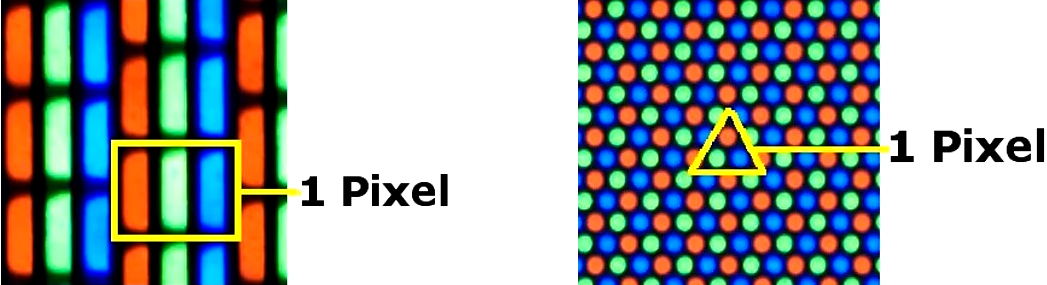
\includegraphics[height=80px]{Pixel_Hardware.png}

Ein Pixel ist i.d.R kein atomarer Baustein eines Hardwaregeräts. Stattdessen besteht er aus i.d.R. 3 Lichtern, welche die 3 Grundfarben ausstrahlen. Wiese das so ist werden wir noch in einem der folgenden Kapitel erfahren, wenn es um Farbmodelle geht.\\
Bei der geometrischen Betrachtung interessieren wir uns für die Form und Anordnung der Bestandteile eines einzelnen Pixels, sowie der Pixel zueinander.

\subsubsection*{Photometrische Betrachtung}
Die Photometrische Betrachtung bezieht sich auf die Darstellung von Objekten mit Farben/Grautönen. Es geht also darum welchen Wert die Pixel annehmen sollen. Dies ist die Betrachtung, die uns im Folgenden beschäftigen wird.

\subsection{Optische Wahrnehmung}
\subsubsection*{Physikalische und Biologische Aspekte}

\begin{wrapfigure}{r}{0.5\textwidth}
    \centering
    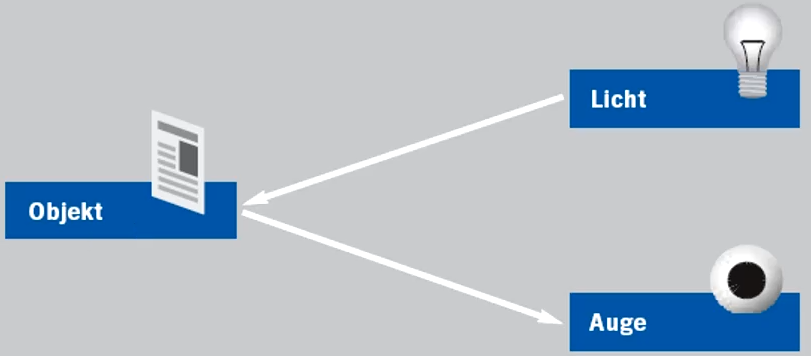
\includegraphics[height=100px]{OptischeWahrnehmung_Reflexion.png}
    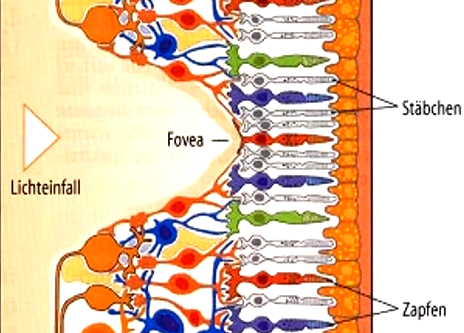
\includegraphics[width=200px]{OptischeWahrnehmung_Retina.png}
\end{wrapfigure}

Objekte werden sichtbar, indem Licht auf sie fällt, reflektiert wird und in unser Auge gelangt. Je nach Oberfläche und Material des Objektes werden unterschiedliche Wellenlängen und damit Farben des Lichtes mehr oder weniger reflektiert. Die nicht reflektierten Lichtstrahlen werden absorbiert und somit in Wärmeenergie umgewandelt.\\

Auf der Retina (syn. Netzhaut) befinden sich Sinneszellen, die Stäbchen und Zapfen. Die Stäbchen sind für das Helligkeitssehen verantwortlich. Die Zapfen gibt es in den 3 Ausprägungen rot, grün und blau. Die Zapfen reagieren hauptsächlich auf die Wellenlänge von licht ihres Typs.\\
Die Empfindlichkeit für Helligkeit ist wesentlich Stärker als die für Farben. Somit können bei wenig Licht fast nur noch die Stäbchen aktiviert werden und wir sehen Nachts bloß schwarz-weiß. Das wird nocheinmal interessant, wenn es um das HSV-Farbmodell geht.

\subsubsection*{Subjektivität der optischen Wahrnehmung}

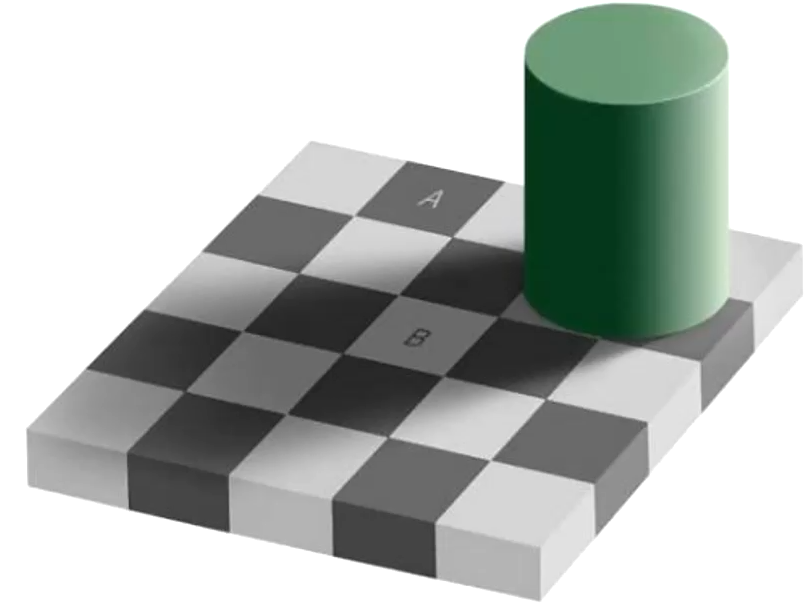
\includegraphics[height=100px]{OptischeWahrnehmung_taeuschungen.png}

Die optische Wahrnehmung ist stark Subjektiv und keinesfalls absolut. Sie wird vor allem durch Erfahrungswerte und neurologische Effekte beeinflusst.\\
Im oberen Beispiel sieht das Feld A viel dunkler aus als das Feld B. Das Gehirn erkennt, dass das Feld B im Schatten liegt und hellt daher seine Farbe auf. Es erkennt auch das Muster des Schachbretts und versucht die Farben so zu interpretieren, dass das Muster nicht gebrochen wird.

\subsection{Farbmodelle}

\subsubsection{CIE Farbraum}
Der CIE Farbraum ist die erste Standardisierung eines Farbraums. Er umfasst alle vom Menschen wahrnehmbaren Farben. Die folgenden Farbmodelle basieren auf diesem Farbraum.

\subsubsection{Hardwareorientiertes Modell - RGB}
\label{sec:RGB}

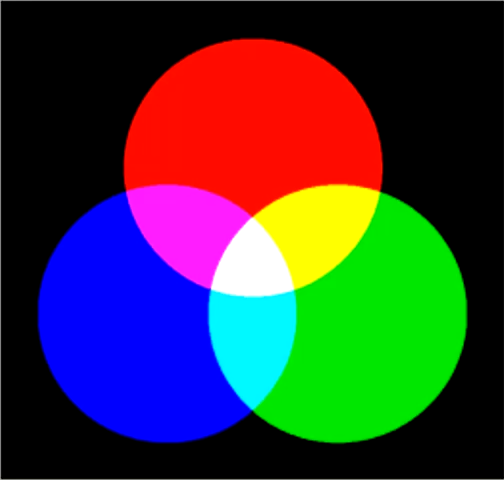
\includegraphics[height=150px]{RGB_circles.png}
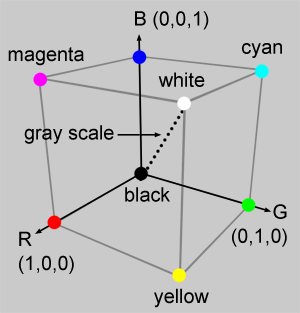
\includegraphics[height=150px]{RGB_cube.png}

Beim RGB Farbmodell besteht jede Farbe aus einer Mischung der 3 Grundfarben \textcolor{red}{rot}, \textcolor{green}{grün} und \textcolor{blue}{blau}. Das bedeutet, dass für jeden Pixel ein Vektor $\vec{v} = \left(\begin{smallmatrix}r \\ g \\ b \end{smallmatrix}\right)$ mit 3 Werten definiert wird.\\
Das RGB Modell ist ein additives Farbmodell. Das bedeutet, dass die Menge an Licht sich bei steigendem Wert einer Komponente des Farbvektors erhöht. Das bedeutet, dass $\vec{v_1} = \left(\begin{smallmatrix}0 \\ 0 \\ 0 \end{smallmatrix}\right)$ schwarz entspricht und ${v_2} = \left(\begin{smallmatrix}1 \\ 1 \\ 1 \end{smallmatrix}\right)$ weiß entspricht.\\
Das additive Farbdenken kennen wir, wenn wir mit Lampen, die verschiedene Farben haben, auf eine weiße Wand leuchten (1. Bild). Das weiße Licht entsteht bei Anwesenheit aller Farben. Entspricht dieses Farbmodell ziemlich direkt der Ansteuerung der einzelnen \hyperref[sec:pixel]{Pixelkomponenten, die wir schon kennengelernt haben}.\\
Die Gerade, die von schwarz nach weiß führt nennt man Unbuntgerade und enthält alle Grautöne. Für Grautöne gilt, dass R=G=B. Das Sechseck, dass aus $\overline{bm}$, $\overline{mR}$, $\overline{Ry}$, $\overline{yG}$, $\overline{Gc}$ und $\overline{cB}$ gebildet wird, enthält alle maximal gesättigten Farben, d.h. Farben mit Sättigung = 100\% \slash 255. Je höher der grauanteil ist (i.e. näher an der Unbuntgerade), desto weniger gesättigt ist die Farbe.\\
\\
In einer Erweiterung des RGB-Modells, dem RGBA-Modell, wird ein weiterer sogenannter Channel angefügt, der sich Alpha-Channel nennt und die Sichtbarkeit bzw. Transparent darstellt. Da wir jeden Channel mit einer genauigkeit von 8Bit darstellen, benötigt RGBA dann 4Byte pro Pixel.

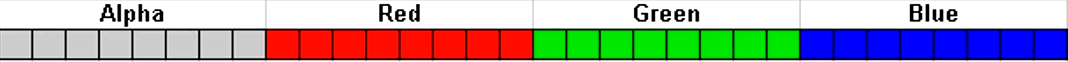
\includegraphics[width=300px]{RGBA.png}

\subsubsection{Hardwareorientertes Modell - CMY}

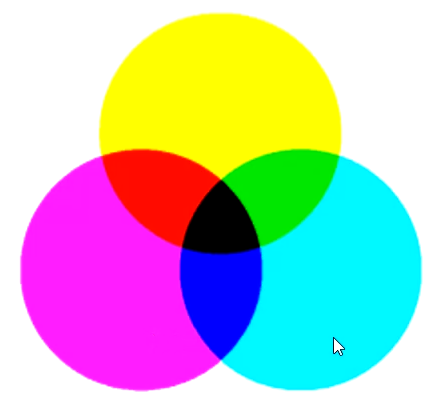
\includegraphics[height=150px]{CMY_circles.png}
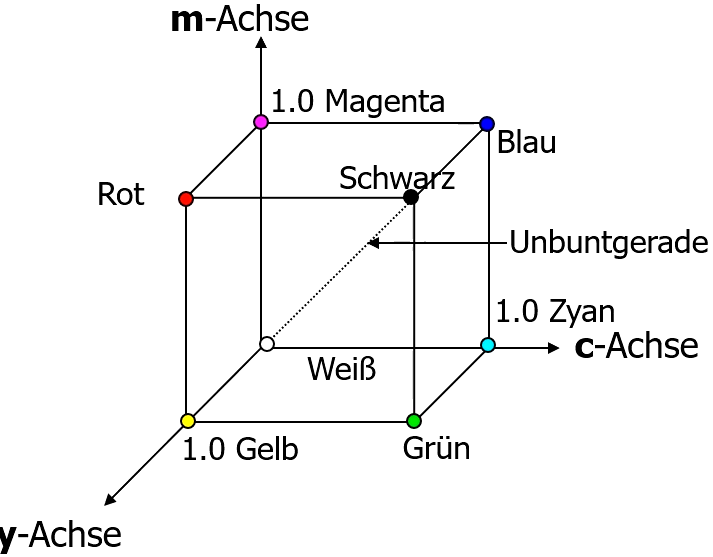
\includegraphics[height=150px]{CMY-cube.png}

Das CMY (Cyan Magenta Yellow) Modell ist ein subtraktives Farbmodell mit den entsprechenden Grundfarben. Umso höher die Werte der Komponenten sind, desto dunkler wird die Farbe, es trifft also weniger Licht ins Auge (subtraktiv). Wir kennen dieses Prinzip beim Mischen von Wasserfarben.\\
Der Farbwürfel des CMY-Modells entsteht aus dem Farbwürfel des RGB-Modells, indem man die Achsenbeschriftung ändert und den Würfel so dreht, dass seine Weiße Ecke im Ursprung liegt.\\
Während das RGB der Lichtmischung entspricht und damit für Displays verwendet werden kann, kann das CMY Modell für Pigmentmischung z.B. beim Drucken verwendet werden.\\
Das \textbf{CMYK} (CMY Blac\textbf{k}) Modell ergänzt das CMY-Modell um einen weiteren Anteil an Schwarz. Der Vorteil dieses Modells ist die bessere Darstellung von Schwaztönen und Konturen z.B. beim Drucken. Eigentlich ist der Black-Channel redundant, da ${v_{CMY}} = \left(\begin{smallmatrix}1 \\ 1 \\ 1 \end{smallmatrix}\right)$ bereits schwarz entspricht. In der Praxis sind die Farben aber nicht perfekt rein, sodass beim Mischen kein perfektes Schwarz entsteht.

\subsubsection{Wahrnehmungorientiertes Modell - HSV}

\begin{wrapfigure}{r}{0.5\textwidth}
    \centering
    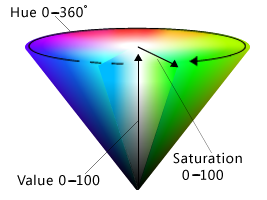
\includegraphics[height=150px]{HSV_room.png}
\end{wrapfigure}

Beim HSV Modell wird eine Farbe in einem Zylinderkoordinatensystem mit den Werten \textbf{H}ue=Farbton (Winkel des Kreisausschnitts 0-365° bzw. 0\% - 100\%), \textbf{S}aturation = Sättigung (Radius des Kreises) und \textbf{V}alue = Helligkeit/Intensität (vertikale Achse) dargestellt. Der Farbverlauf des oberen Randes des Farbkegels entspricht genau dem Sechseck der maximal gesättigten Farben des \hyperref[sec:RGB]{RGB-Würfels}.\\
Im folgenden sehen wir ein Beispiel für die Zerlegung eines Farbbilds in die 3 HSV Kanäle, wobei jeder extrahierte Wert $x \in [0, 1]$ wieder als Wert eines schwarz-weiß Bildes interpretiert wird, wobei 0 schwarz entspricht und 1 weiß.\\
Die Bilder sind in der Reihenfolge All, \textbf{S}aturation, \textbf{V}alue, \textbf{Hue} gezeigt:

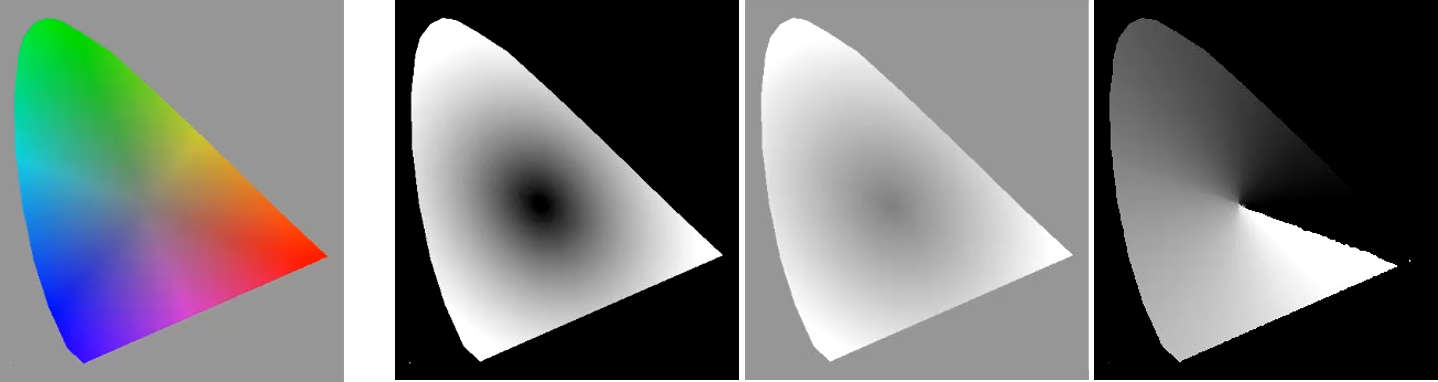
\includegraphics[height=100px]{HSV_decomposition.png}

\textbf{Erklärung der Zuordung:}\\
Auf dem \textbf{ersten Bild} ist der graue Hintergrund schwarz, da die Sättigung von Grautönen Null ist. Außerdem ist die Außenkante des Objektes weiß, da hier die maximal gesättigten Farben liegen. Somit handelt es sich um die Saturation.\\
Auf dem \textbf{zweiten Bild} ist der Hintergrund identisch mit dem grauen Hintergrund vom Originalbild, denn Ein Grauton entspricht in HSV einem puren Helligkeitswert. Somit handelt es sich um Value.\\
Auf dem \textbf{dritten Bild} ist der Hintergrund schwarz, da Grautöne in HSV keinen Farbwert haben. Außerdem zeigt sich der Farbverlauf als lineare Steigerung der Graustufen, da die Farben genau so angeordnet sind, wie sie im HSV-Farbkegel angeordnet sind. Somit steigt der Wert des ihnen zugeordneten Winkels stetig.\\
\\
Da das HSV-Modell die Farben getrennt von der Helligkeit speichert, konnte mithilfe dieses Modells früher (in der Zeit des Schwarz-Weiß-Fernsehens) einfach ohne Rechnen aus einem Farbfilm ein Schwar-Weiß-Film extrahiert werden, der an private Haushalte ausgestrahlt werden konnte.\\
Außerdem können manche Algorithmen der Bildverarbeitung schneller mit solchen Bildern arbeiten, da viele Techniken hauptsächlich auf Helligkeitswerten basieren.

\subsubsection{YUV Farbmodell und 4:1:1 Farbraum}

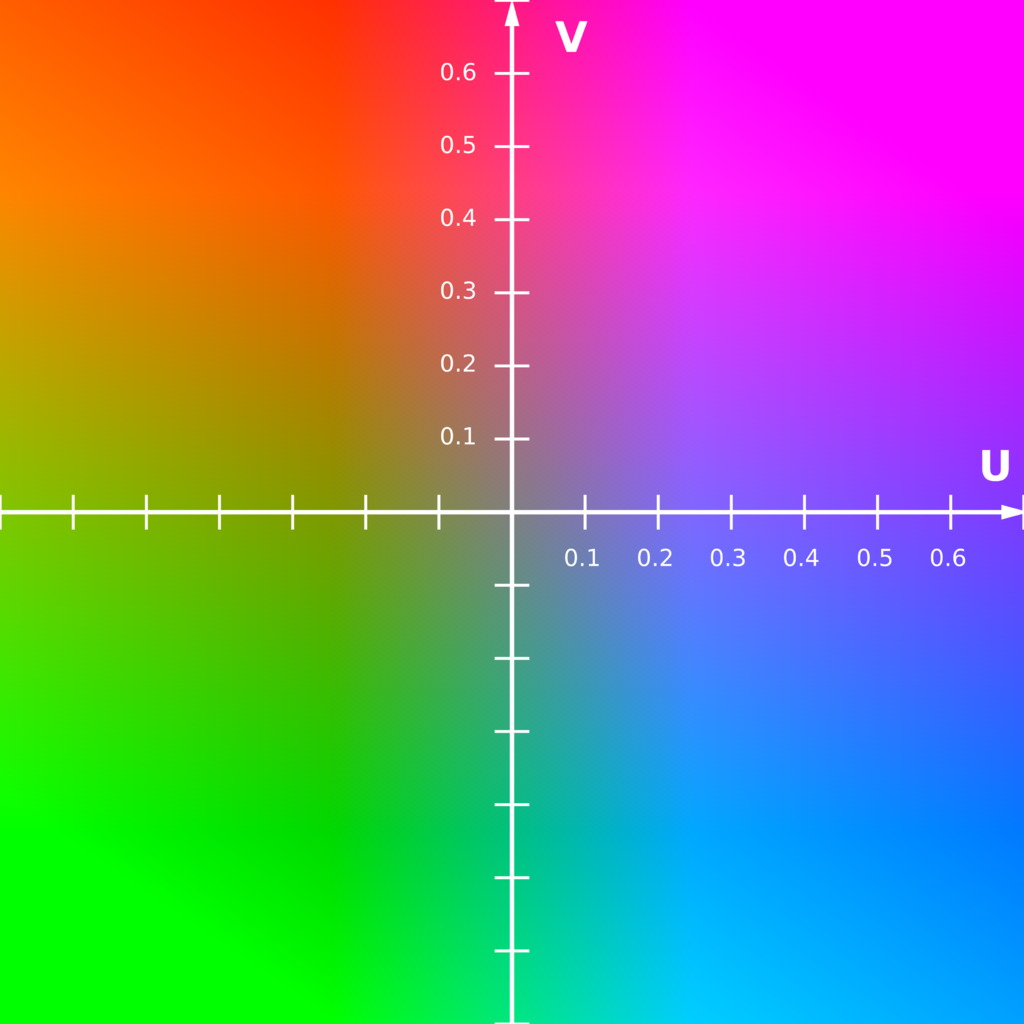
\includegraphics[height=150px]{YUV.png}

Im YUV-Farbmodell wird eine Farbe mittels eines Chrominanz-Wertes, der aus 2 sättigungslosen Farben U und V (siehe Bild) besteht, und einem Luminanzwert (Helligkeit) bestimmt.\\
Dieses Modell kann benutzt werden, um Bilder zu komprimieren. Denn das menschliche Auge ist sehr viel empfindlicher für Helligkeit als für Farbe. Somit kann man, wenn die Farbe und Helligkeit getrennt gespeichert sind, weniger Daten für die Farbe als für die Helligkeit benutzen, ohne dass es für dem Menschen wahrnehmbar ist. Oft wird der sog. 4:1:1 Farbraum verwendet, in dem für 4 Pixel auch 4 Helligkeitswerte gespeichert werden, aber nur 1 Farbwert U und ein Farbwert V.